%-----------------------------------------------------------------------------------------------%
%
% Maret 2019
% Template Latex untuk Tugas Akhir Program Studi Sistem informasi ini
% dikembangkan oleh Inggih Permana (inggihjava@gmail.com)
%
% Template ini dikembangkan dari template yang dibuat oleh Andreas Febrian (Fasilkom UI 2003).
%
% Orang yang cerdas adalah orang yang paling banyak mengingat kematian.
%
%-----------------------------------------------------------------------------------------------%

%-----------------------------------------------------------------------------%
%\prefikLampiran{A}

\renewcommand{\thepage}{B - \arabic{page}}
\chapter{HASIL OBSERVASI}
%-----------------------------------------------------------------------------%
\begin{figure}
	\centering
	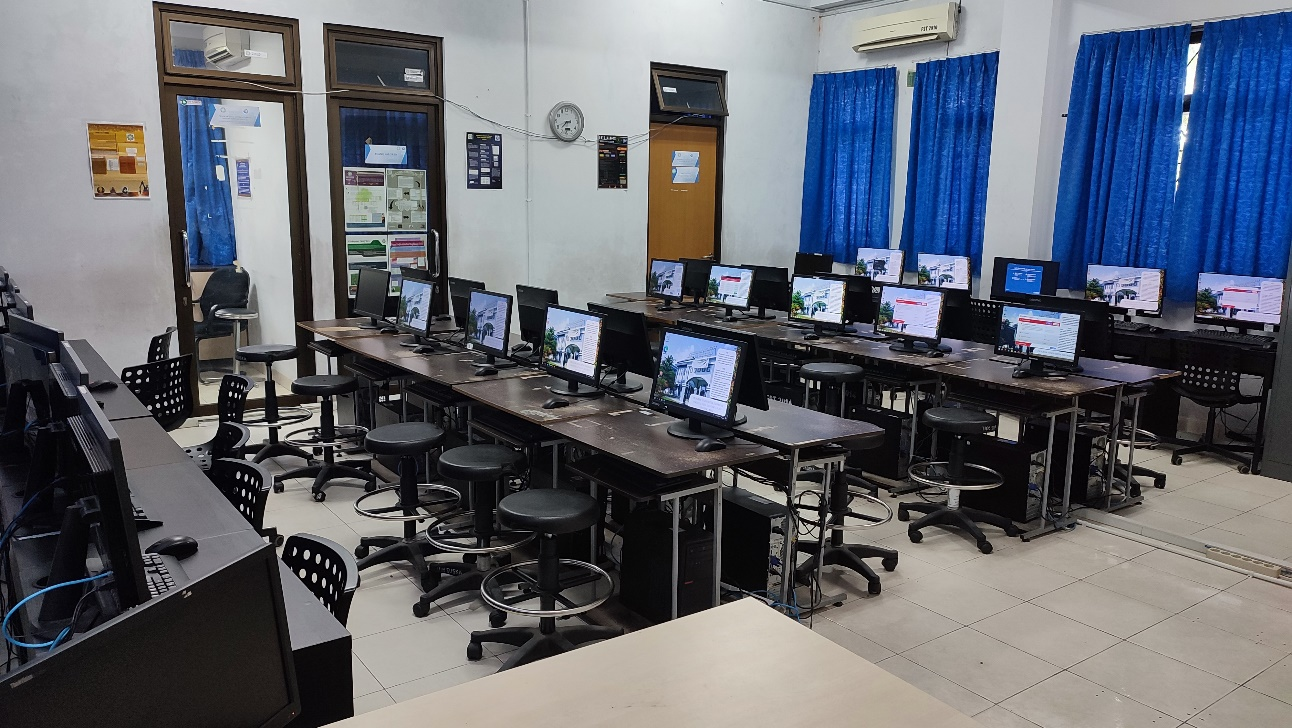
\includegraphics[width=0.82\linewidth]{konten/gambar/lab-rsi.jpg}
	\caption{Laboratorium Rekayasa Sistem Informasi \protect\cite{labsi2023}}
	\label{fig:lab-rsi}
\end{figure}

\begin{figure}
	\centering
	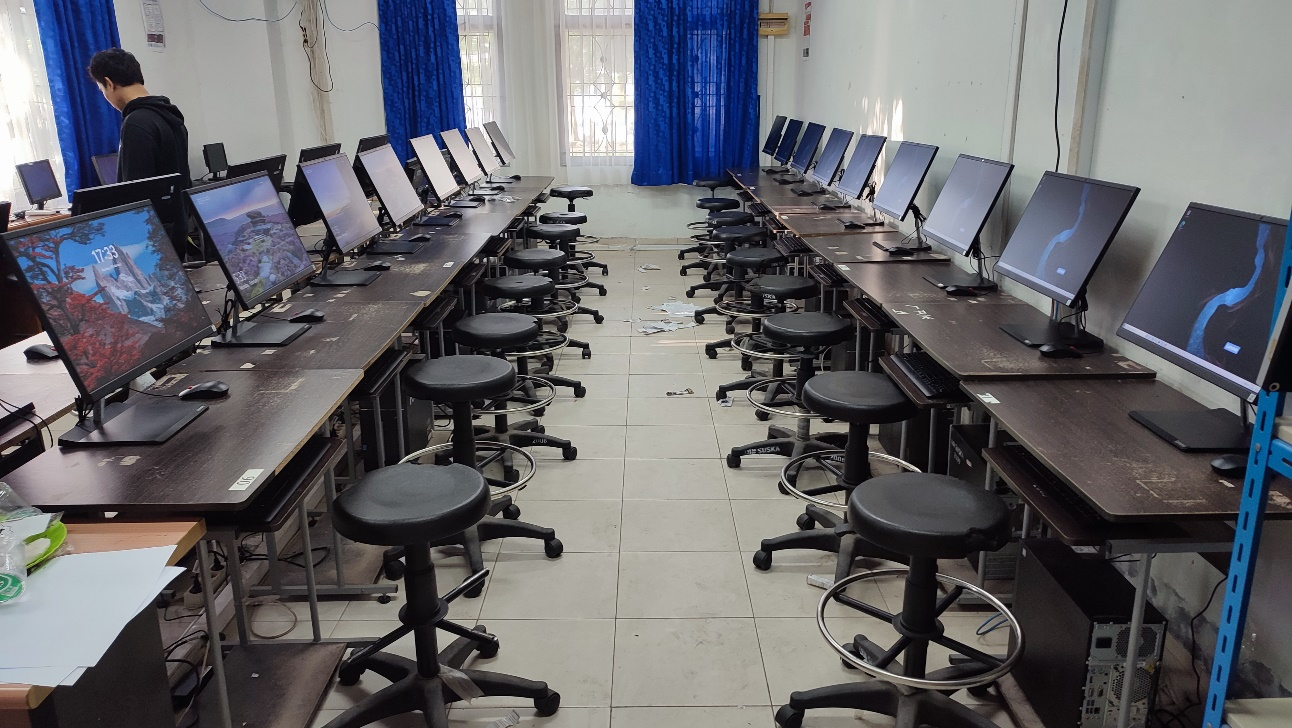
\includegraphics[width=0.82\linewidth]{konten/gambar/lab-internet.jpg}
	\caption{Laboratorium Internet \protect\cite{labsi2023}}
	\label{fig:lab-int}
\end{figure}

\begin{figure}
	\centering
	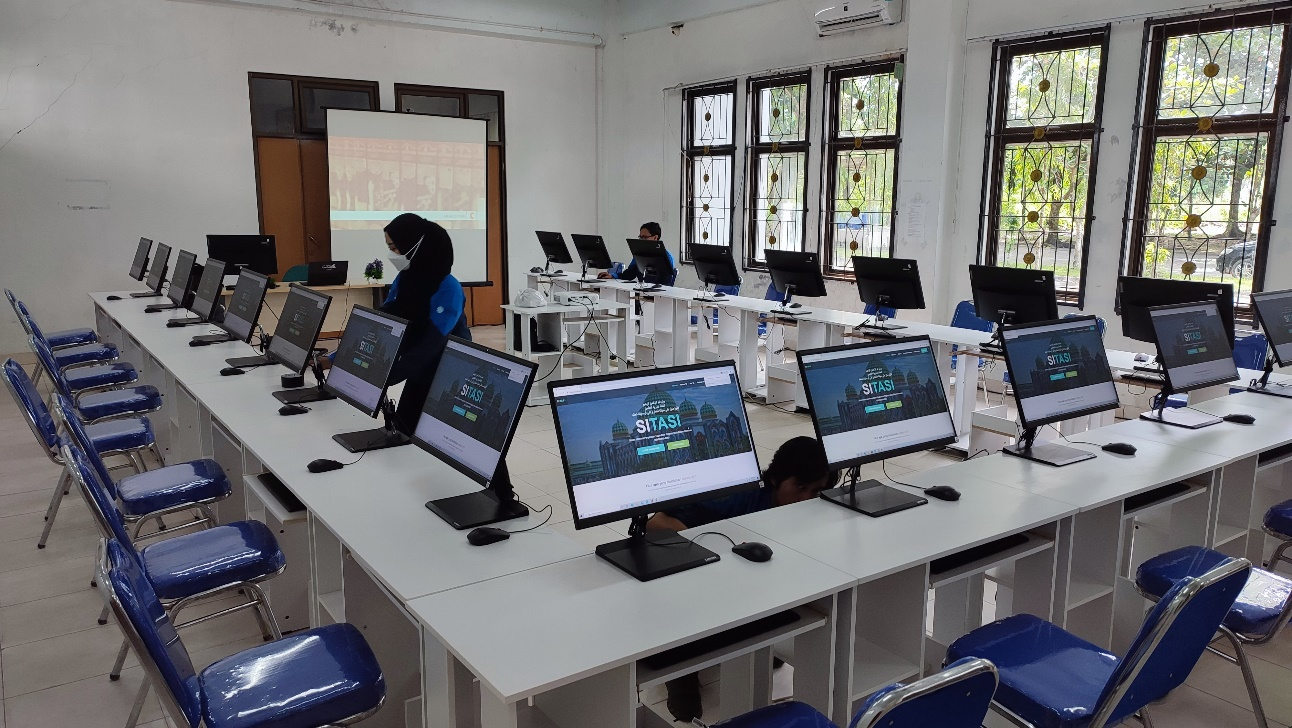
\includegraphics[width=0.82\linewidth]{konten/gambar/lab-se.jpg}
	\caption{Laboratorium Internet \protect\cite{labsi2023}}
	\label{fig:lab-int}
\end{figure}

\begin{figure}
	\centering
	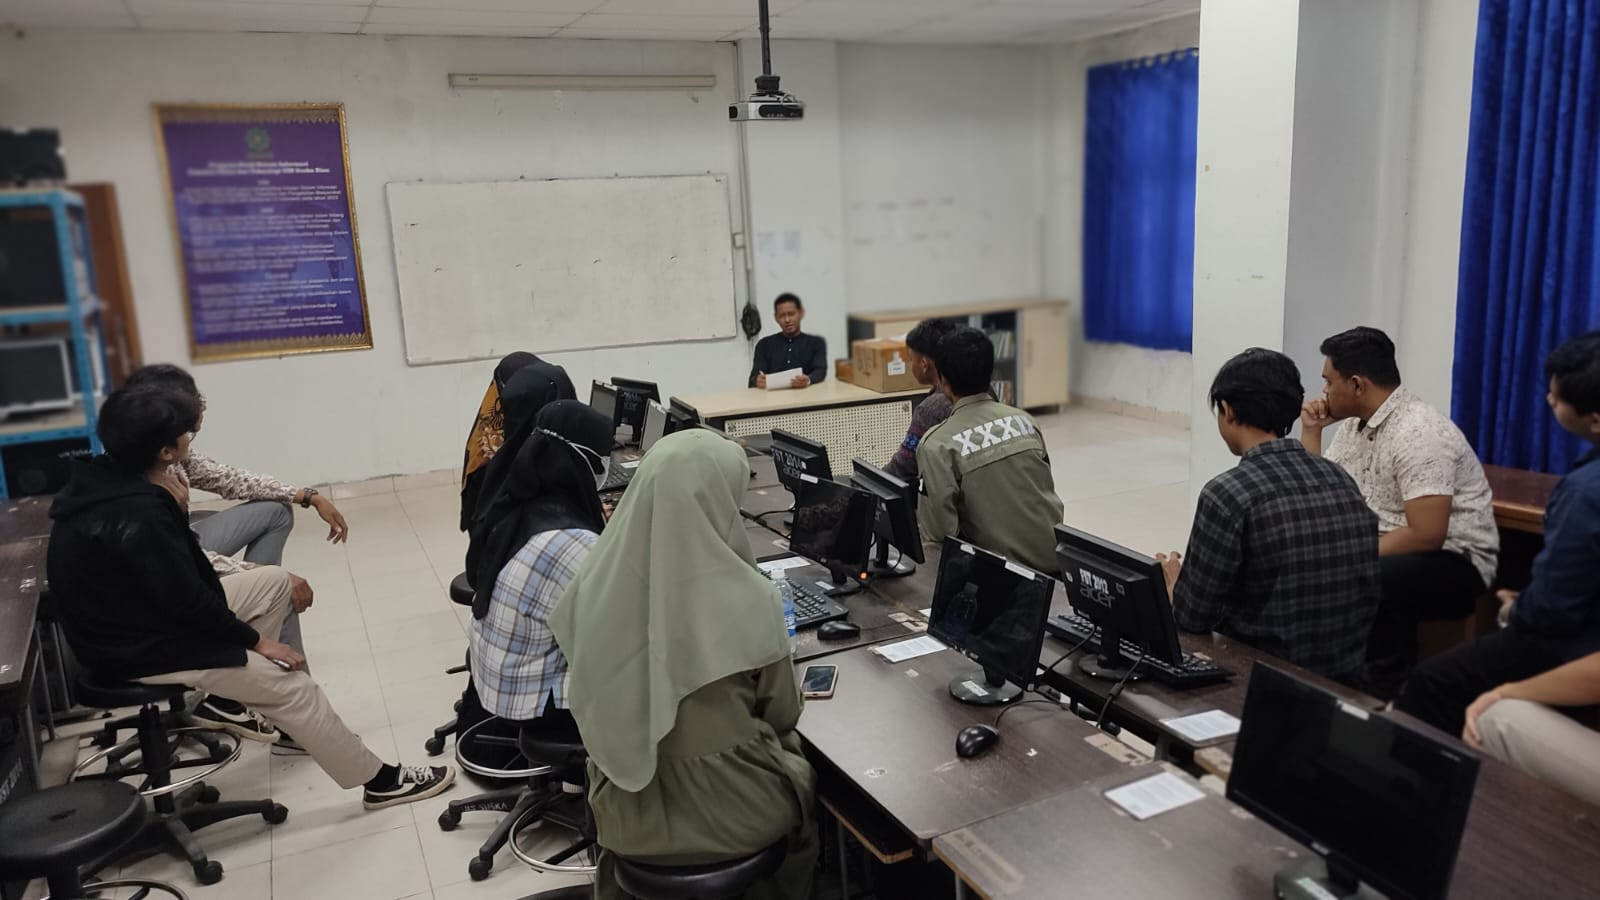
\includegraphics[width=0.82\linewidth]{konten/gambar/kegiatan.jpg}
	\caption{Kegiatan Laboratorium} \protect\cite{labsi2023}
	\label{fig:lab-sea}
\end{figure}

\begin{figure}
	\centering
	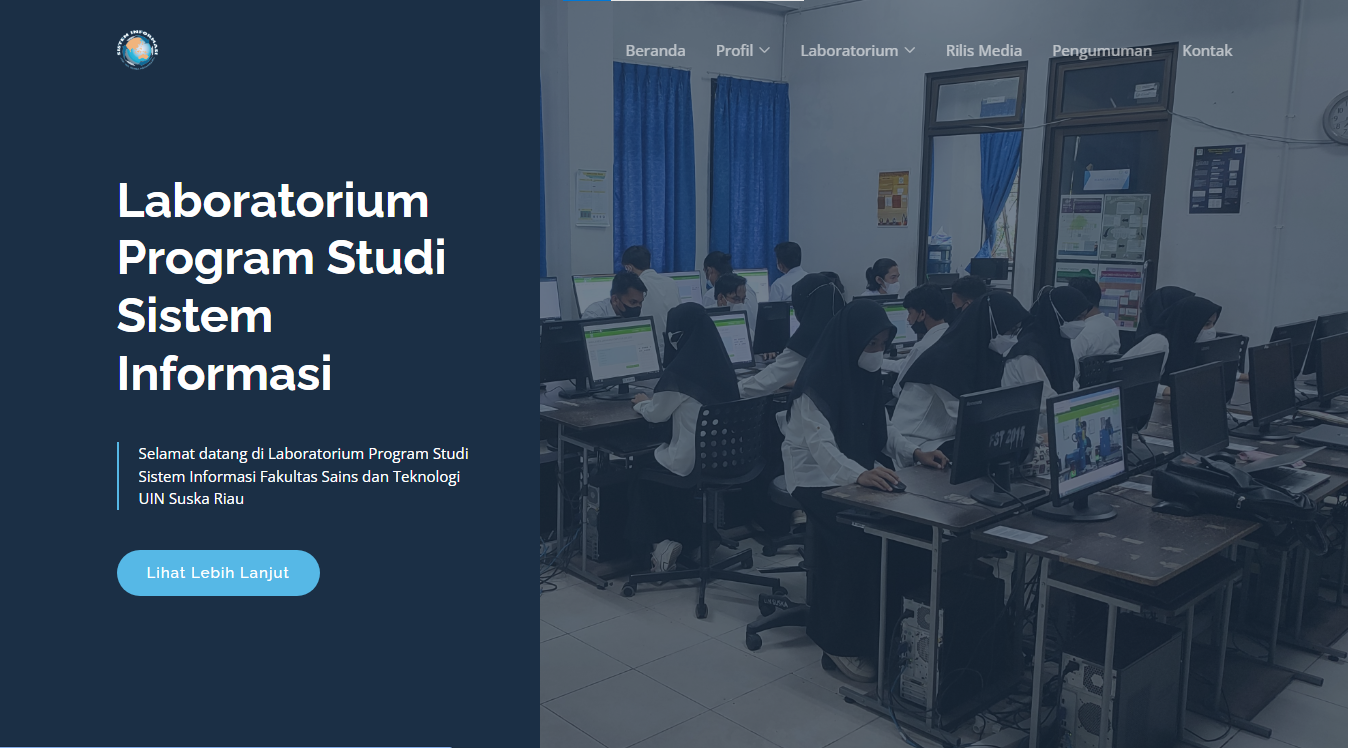
\includegraphics[width=0.82\linewidth]{konten//gambar/labsi.png}
	\caption{Website Laboratorium Program Studi Sistem Informasi \protect\cite{web-prodi}}
	\label{fig:enter-label}
\end{figure}

\begin{figure}
	\centering
	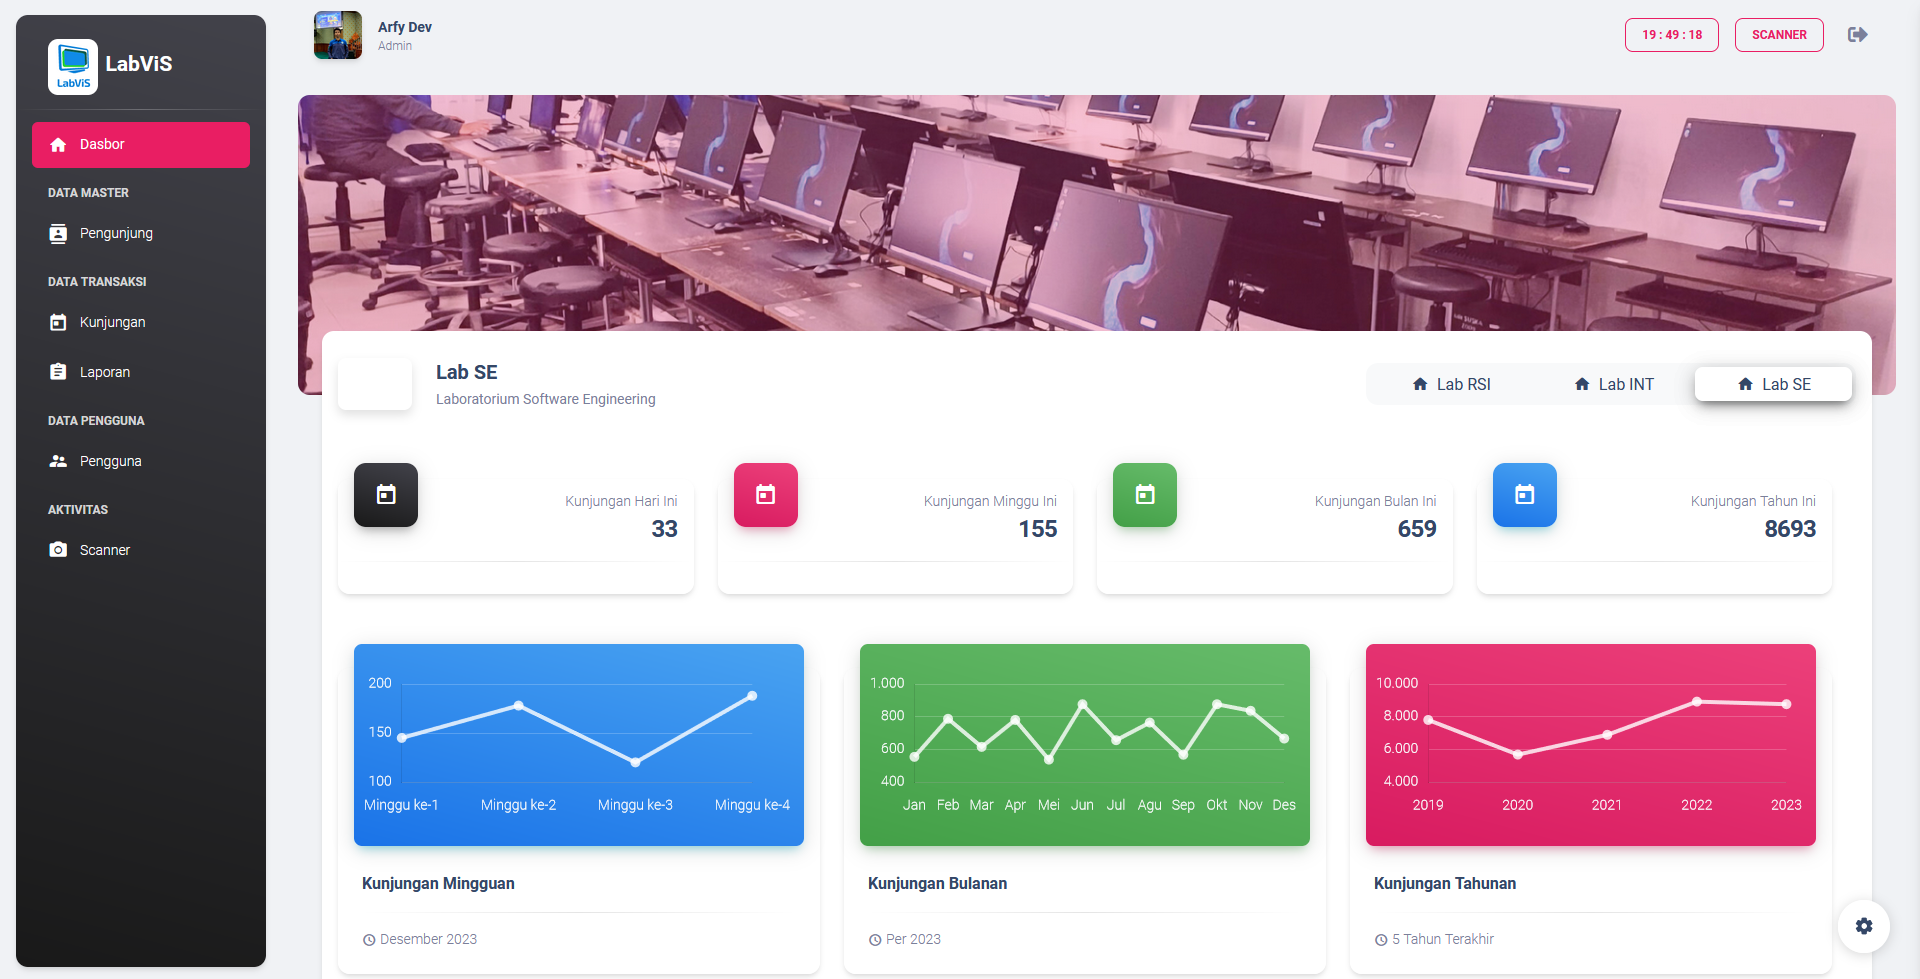
\includegraphics[width=0.82\linewidth]{konten//gambar/labvis.png}
	\caption{\textit{Laboratory Visitor System (LABVIS)} \protect\cite{web-prodi}}
	\label{fig:enter-label}
\end{figure}

\begin{figure}
	\centering
	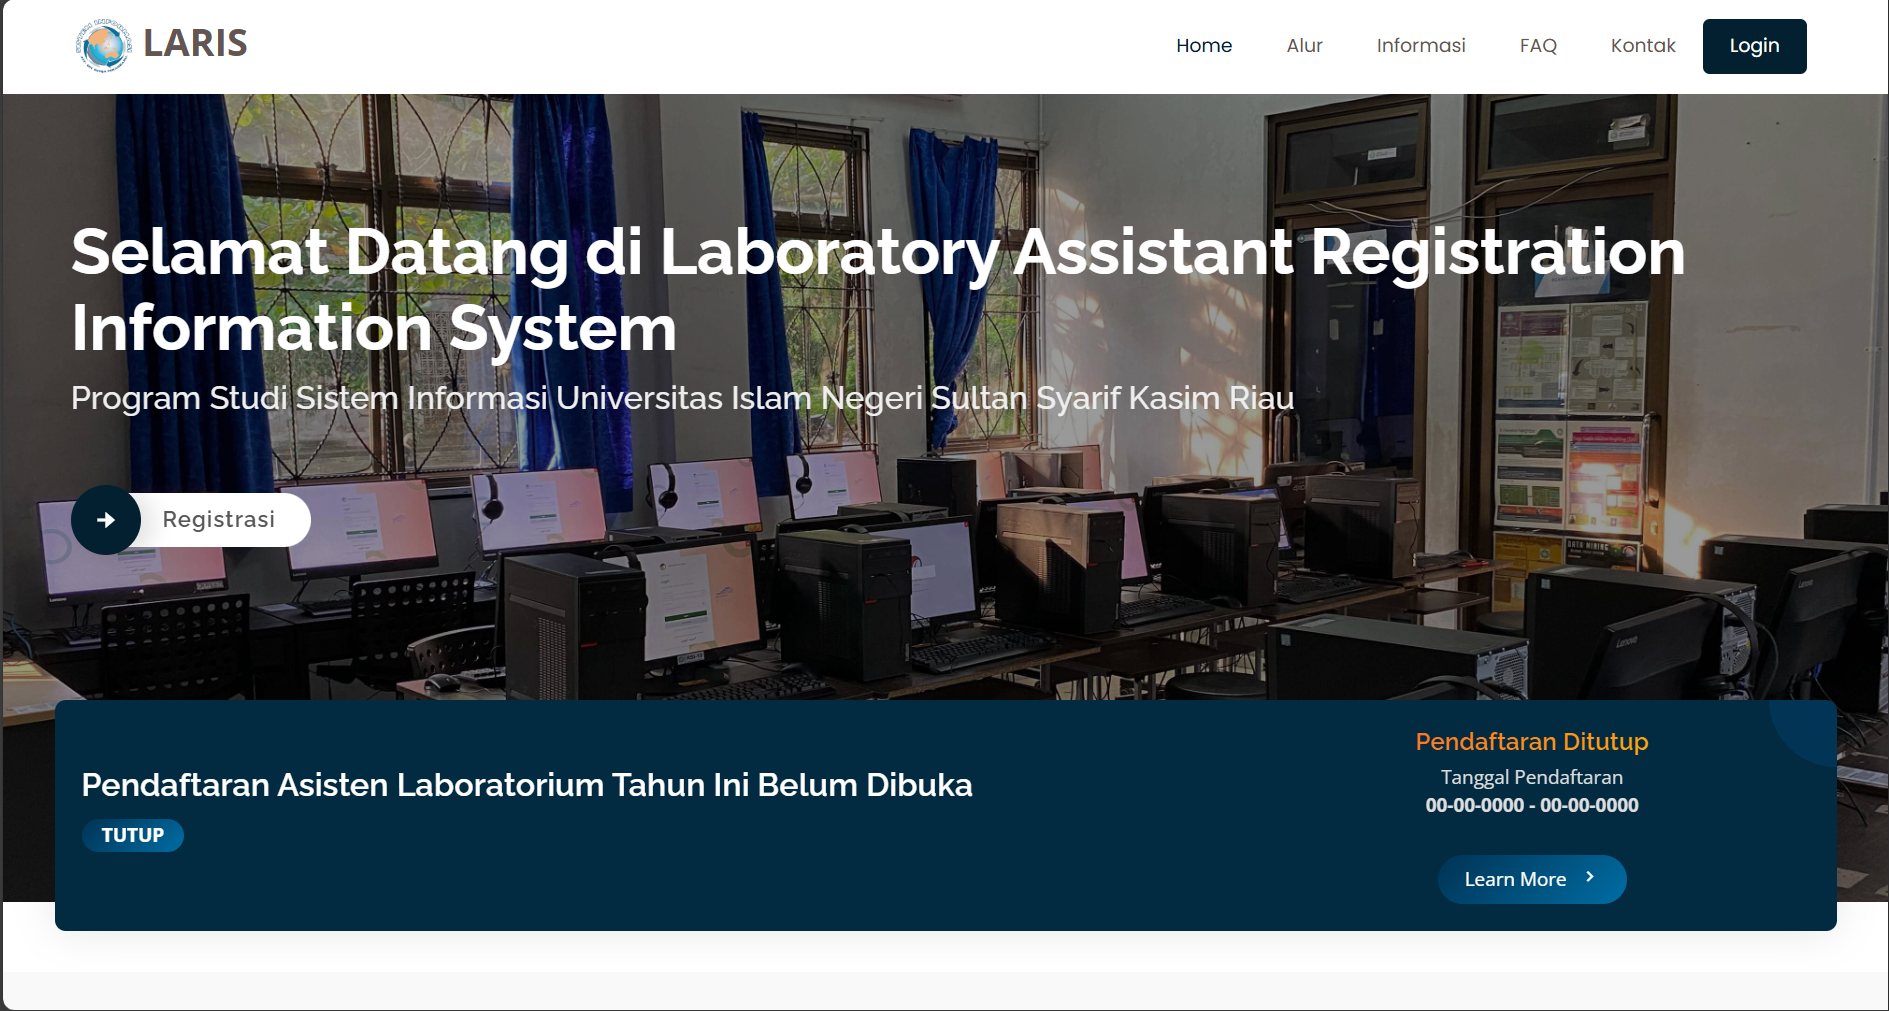
\includegraphics[width=0.82\linewidth]{konten//gambar/laris.png}
	\caption{\textit{Laboratory Assistant Registration Information System (LARIS)} \protect\cite{web-prodi}}
	\label{fig:enter-label}
\end{figure}

\begin{figure}
	\centering
	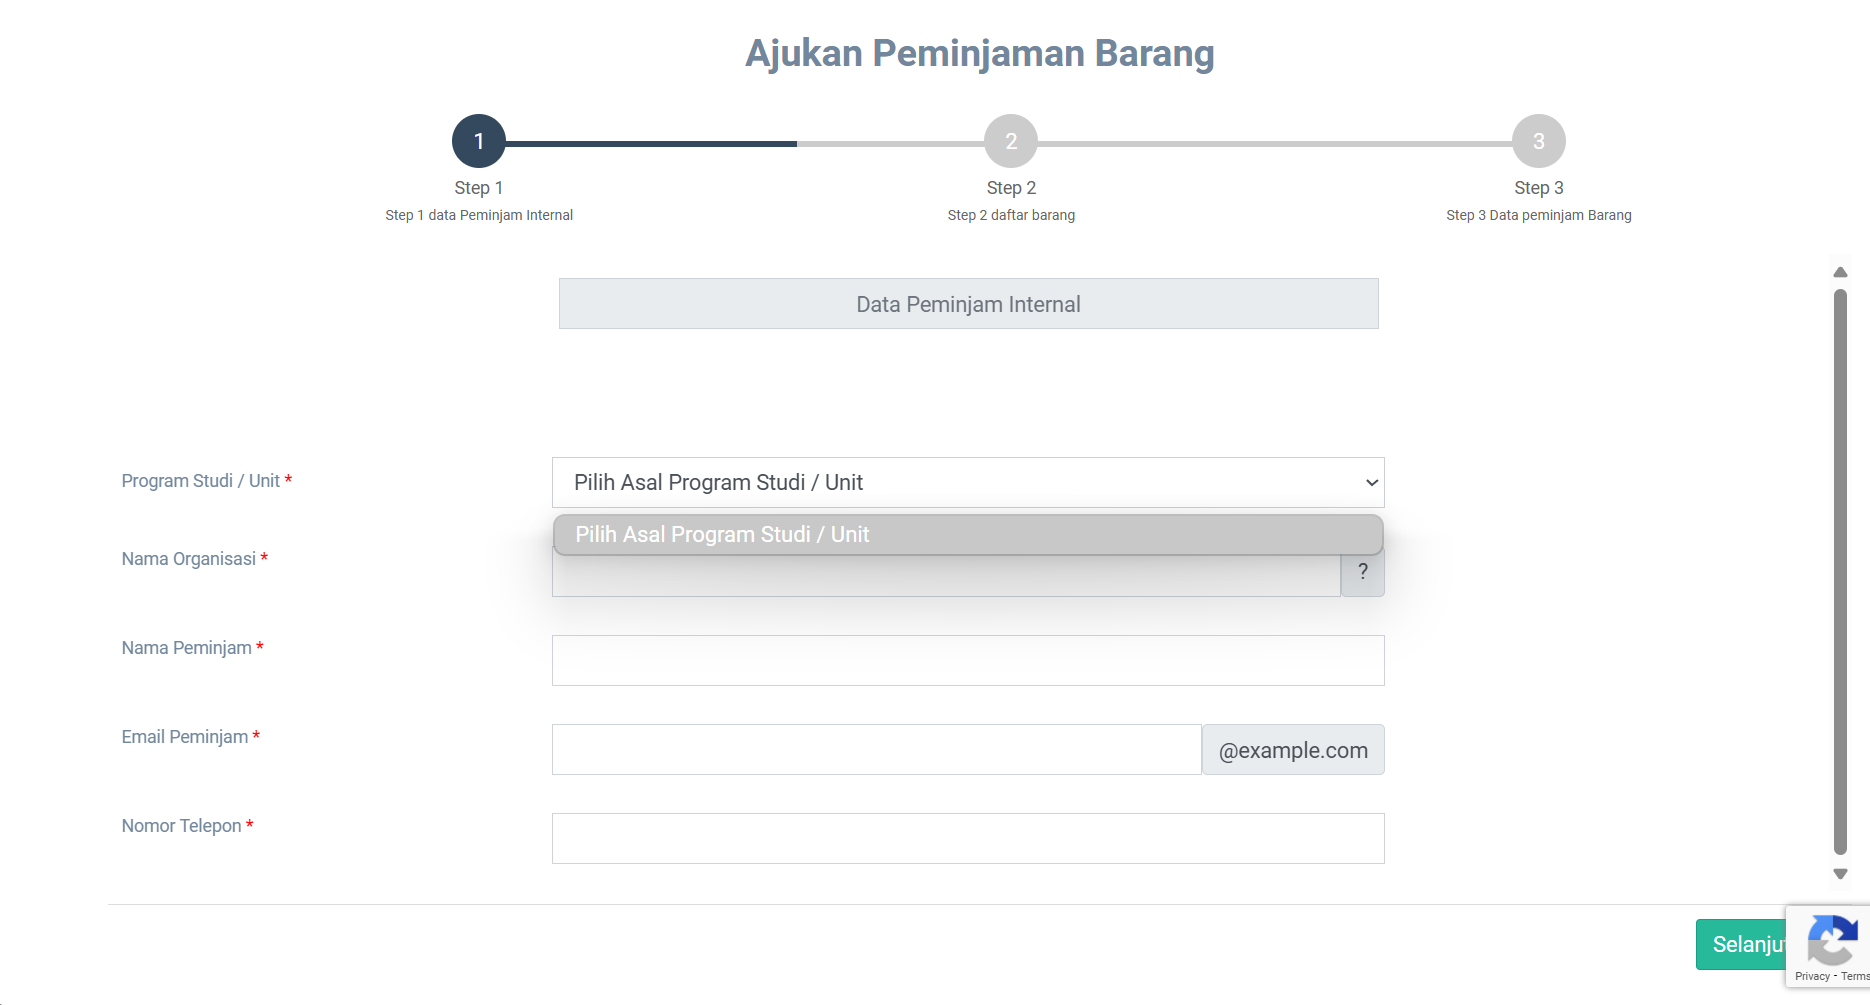
\includegraphics[width=0.82\linewidth]{konten//gambar/observasi-peminjaman-barang.png}
	\caption{Disfungsi Fitur Peminjaman Barang} \protect\cite{sitaris}
	\label{fig:enter-label}
\end{figure}

\begin{figure}
	\centering
	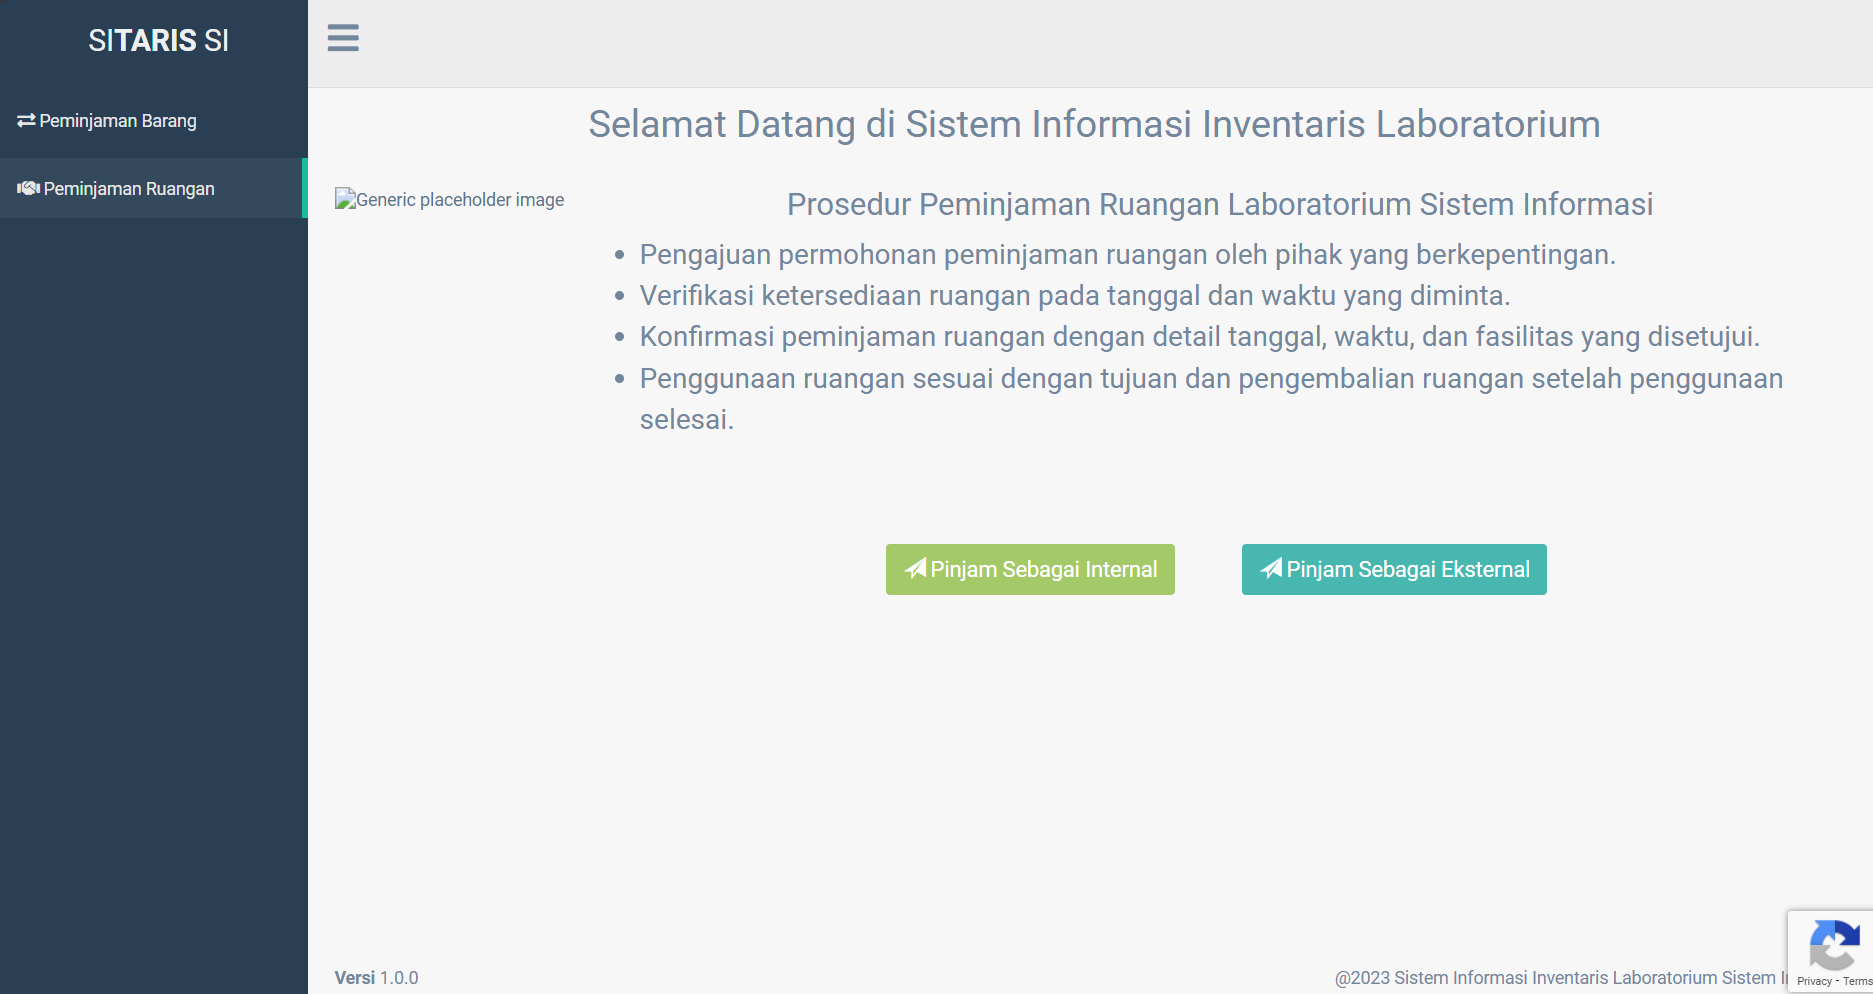
\includegraphics[width=0.82\linewidth]{konten//gambar/observasi-peminjaman-ruangan.png}
	\caption{Disfungsi Fitur Peminjaman Ruangan} \protect\cite{sitaris}
	\label{fig:enter-label}
\end{figure}

\begin{figure}
	\centering
	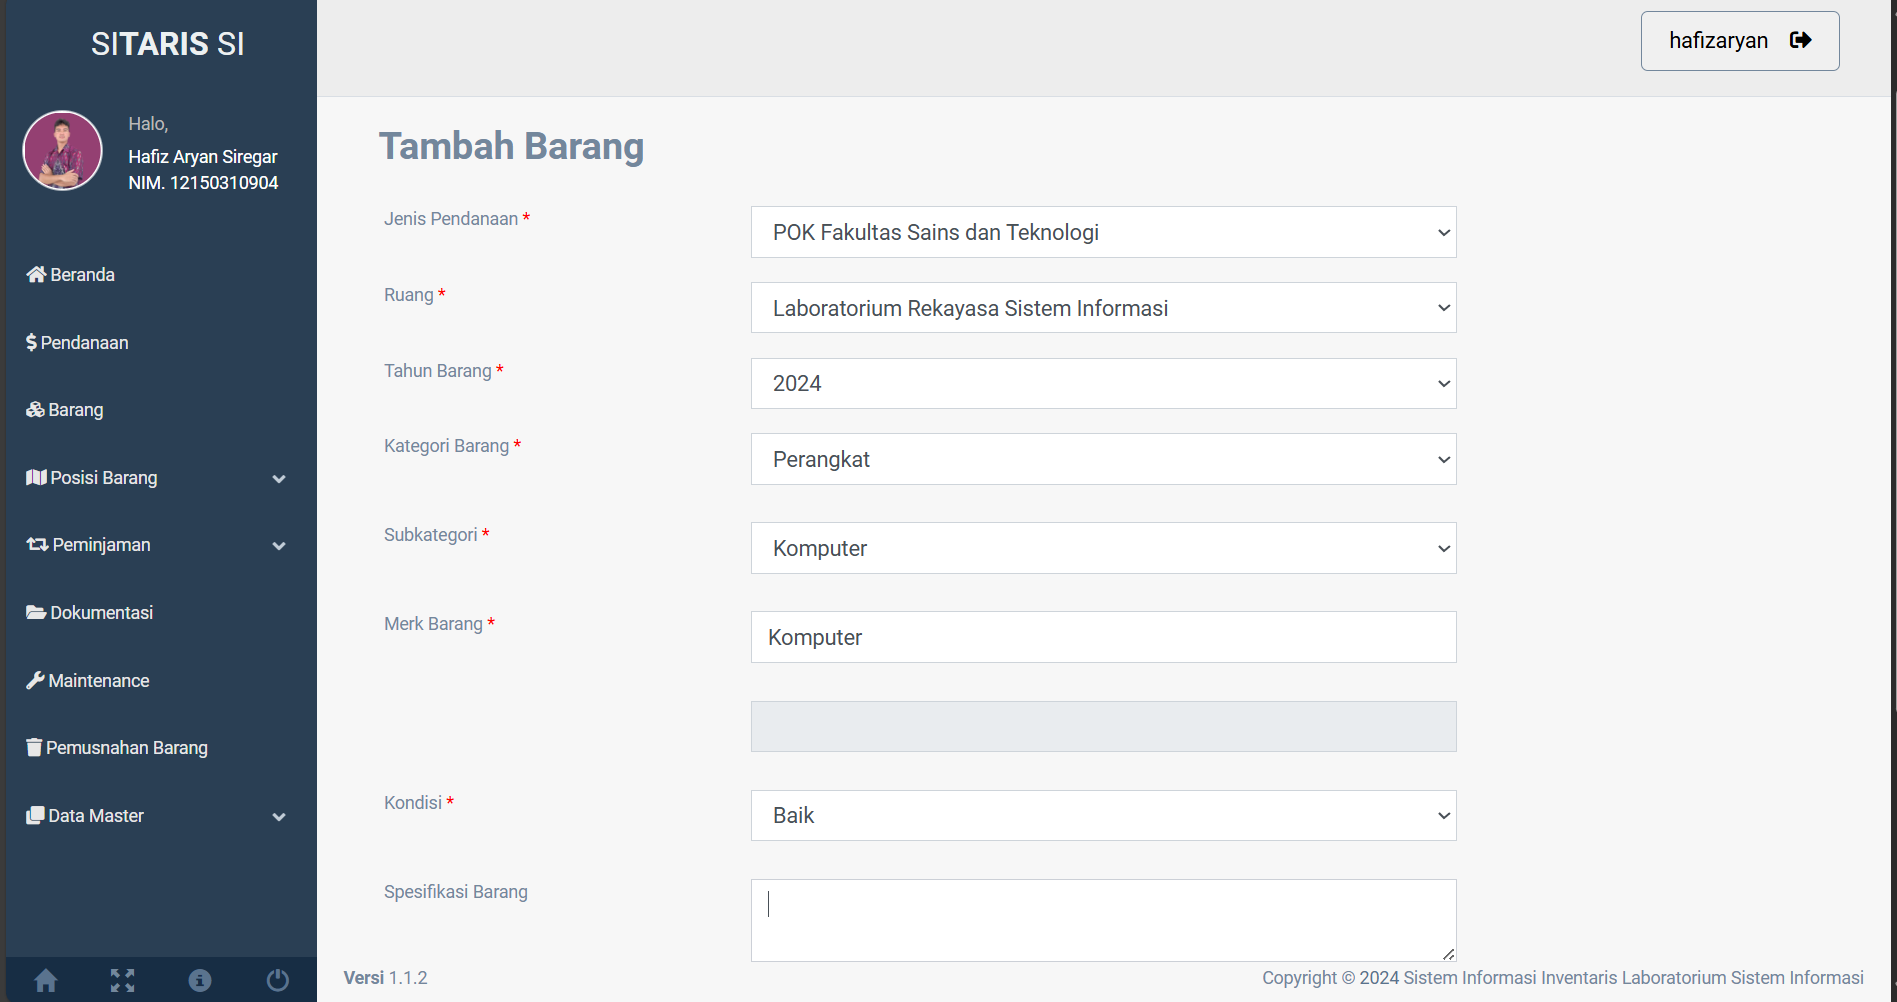
\includegraphics[width=0.82\linewidth]{konten//gambar/kode-barang.png}
	\caption{Disfungsi Pembuatan Kode Barang} \protect\cite{sitaris}
	\label{fig:enter-label}
\end{figure}